\section{TinyDAS}

In this section, we introduce TinyDAS, a Python program aimed at training autoencoder models and detecting anomalies within \acrshort{das} data. 

\subsection{Tools}
\mycomment{
Python is a dynamically typed, weak language famously known for it's \textit{easy-to-learn} syntax. Created by Guido Van Rossum in the late 80-s \cite{python}, Python has slowly emerged as one of the fastest growing programming languages ever created \cite{srinath2017python}. 

Virtually all of the larger libraries for data science and \acrlong{ml} have bindings to \gls{python}, or are written in Python from scratch. Some examples include \texttt{Pandas}, \texttt{NumPy}, \texttt{SciKit Learn}, \texttt{Pytorch} and \texttt{TensorFlow}. Many of these rely on code written in C or C++ to be fast, sincc
}

In addition to \texttt{Tinygrad}, we will also be utilizing \texttt{Pytorch} for certain models, as \texttt{Float16} calculations appear to be a bit more stable for certain models. For anomaly detection, we utilize several popular Python packages such as \texttt{numpy}, \texttt{scikit-learn} and \texttt{seaborn} for evaluation metrics, and \texttt{matplotlib} for visualization and plots. A full list of packages used can be found in 
appendix \ref{app:tinypacks}.


\subsection{Overview}

TinyDAS consists of two parts. The first part handles model construction and training, while the latter deals with anomaly detection of \acrshort{das} data. An overview of how TinyDAS works is shown in figure \ref{fig:dataflow}. The following list outlines the fundamental philosophies and criteria used to design and evaluate the framework:

\begin{figure}[!h]
    \centering
    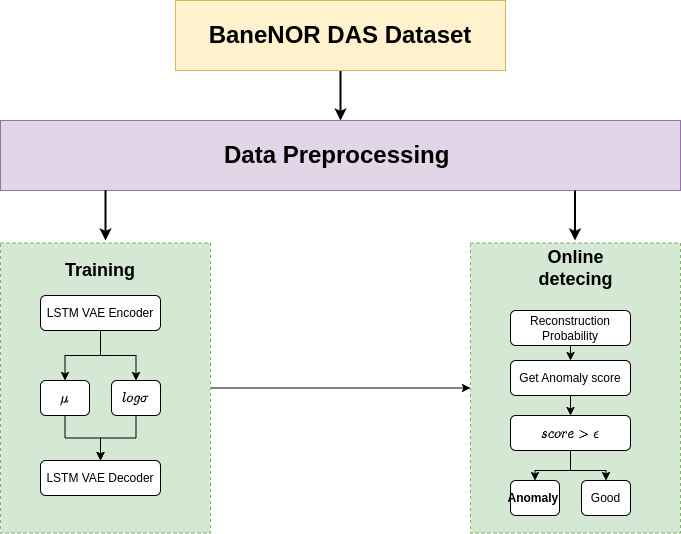
\includegraphics[scale=0.5]{figures/methodflow.png}
    \caption{Overview of TinyDAS}
    \label{fig:dataflow}
\end{figure}


\begin{enumerate}
    \item \textit{Support} for memory-efficient training techniques, specifically half-precision
    \item \textit{Scalability} from single-core systems to multi-node clusters
    \item \textit{Hardware agnostic} to ensure wide usability
    \item \textit{Modular architecture}, easily extendable with new models
    \item \textit{Separation of core logic} from data workflow for improved maintainability
    \item \textit{Collection} of different algorithms for anomaly detection
    \item \textit{Future potential} for online anomaly detection in a live environment
    \item \textit{Model-agnostic} approach to anomaly detection for broader applicability
\end{enumerate}

\subsection{Models} 

We implementing four types of autoencoders: a linear autoencoder (AE), a convolutional autoencoder (CAE), a variational autoencoder (VAE), and a convolutional variational autoencoder (CVAE). The first model serves as a baseline to test against. In AE models, the latent space $Z$ can become disjoint and non-continuous, which VAE models try to solve. Additionally, we introduce convolutional layers in an attempt to improve the model's feature extraction capabilities. Based on this, these models serve as a baseline for what is to be expected by autoencoders for anomaly detection. A full list of layers and parameter sizes can be found in the appendix \ref{app:archs}. \\

\subsection{\acrshort{api} design}

Due to Tinygrad being a relatively simple framework, we implement components to be used for training and testing, with the intent of being reusable and modular.

\subsubsection{Datasets and Dataloaders}

The \texttt{Dataset} and \texttt{DataLoader} classes supports reading in \acrshort{hdf5} in batches, with support for data normalization and type casting. The former handles information about the dataset to be trained on, as well as logic for loading a single file from a \acrshort{hdf5} file, or whatever other format might be sent in later on. The latter one handles loading of batches in parallel, loading $n$ samples into the model.

\subsubsection{Autoencoder Base Class}

\lstinline{BaseAE} is the abstract class which all the different models inherit from. As long as all models inherits from this class, it will be run in the trainer. The \lstinline{criterion} method is the main method to call when training a model. It runs the \lstinline{__call__} method, applies the loss function of choice, and stores in a dictionary in case we'd like to save multiple losses across epochs. We define the class as follows:

\lstinputlisting[language=Python, label={lst:baseae}, caption=Base Autoencoder class]{code/baseae.py}

\subsubsection{Early Stopping}

As of now, we do not use a validation dataset for our training, so we will instead be using the training loss as a trigger. This will of course not allow us to analyze our hyperparameters, but will 

\lstinputlisting[language=Python, label={cods:es}, caption=Early Stopping Mechanism]{code/es.py}

For each epoch in our training lop

\subsubsection{Trainer}

The Trainer class serves as the core component of our program. As demonstrated in listing \ref{fig:lstmcell}, it integrates a model, dataloader, and optimizer to execute the training process. Additionally, it handles early stopping, storing history of losses and saving the best model for further use. The core functions of the \texttt{Trainer} class is shown in code listing \ref{code:trainer}.

\lstinputlisting[language=Python, caption=Core function snippets of the \texttt{Trainer} class, label={code:trainer}]{code/trainer.py}

One of the more important aspects of this class is the \texttt{train} function, which leverages the \acrshort{jit} compiler to replay this kernel for each iteration, resulting in faster training times. Furthermore, the \texttt{reshape\_fn} lambda function allows us to reshape data based on if our model is convolutional or not. For convoluional models, input should be $[BS, C, H, W]$ and $[BS, H, W]$ for models with linear input, where $BS$ is batch size, $C$ is amomunt of channels (always 1 for our \acrshort{das} data), and $H$ and $W$ is height and width of the matrix. This is not done in the model itself due to some instability with the \texttt{Tinygrad} \acrshort{api}. We continuously check and store the trainable parameters of the best performing models.


\subsection{Usage}

\subsubsection{Training}

In the same way that \texttt{Judas} is designed, we want \texttt{TinyDAS} to be modular and easy to use. We've designed components in a way that is familiar to that of \texttt{Pytorch}. Models can be trained using the following script:

\lstinputlisting[caption=Example of how models within \texttt{TinyDAS} is trained, language=Python]{code/tinydas_main.py}

We allow for \texttt{Float16} training by type casting all weights and biases in the model, which effectively halves the memory requirement.

\subsubsection{Hyperparameters and configurations}

Hyperparameters for the different models are stored in separate YAML files. A full overview can be found in appendix \ref{app:configs}.


\subsubsection{Anomaly Detection}

After having trained the models on normal signal data, we move on to the anomaly detection section of our program. As mentioned in \ref{back:anomdet}, first decide which types of anomalies are to be found. We decided to first of all split the files into smaller files of \qty{5}{\si{\second}} files, partially to fascilitate for faster inference of our model. We decide to look at the whole array as whole, instead of finding segments. We will be calculating precisions, recalls and f1scores to find a threshold for reconstruction loss of our data to determine whether or not the data is anomalous. In code listing \ref{code:th}, a function for finding this threshold is presented.  \\

\lstinputlisting[language=Python, caption=Code for finding the best threshold, label={code:th}]{code/bestth.py}

By finding the optimal threshold, we can utilize this in an online environment, preprocessing incoming \acrshort{das} data to fit our model and mark the data as anomalous if \lstinline[language=Julia]{reconstruction_error > threshold}. 

Clustering + LabelFree Detection for discussion? reconstruction error per cell and a clustering algorithm could find where in the signal the anomaly is found

